%
\chapter{Introduction}\label{ch:background}
%
\section{Gene expression in complex tissues}\label{sec:gene_expression_background}
     
          \subsection{Spatial organization of complex biological tissues like the brain}
     This section meant to ask some of the fundamental questions that intrinsically motivate the work presented in the rest of this thesis. Complex tissues, the most obvious example of which is the brain, can be viewed as an interconnected mosaic of cells having different functions, working together to achieve the global function of the organ.\\
     
     When looking closely at this mosaic of cells, it is easy to observe that the spatial organisation is not random. Indeed, cells that serve the same function will often be close to each other, thus defining functional tissues. However, the spatial coherency of those tissues is not necessarily always the same. Some cell types may consist of cells that are scattered inside another more spatially coherent tissue. To illustrate this, an interesting example is the difference between the spatial coherency of cells forming the neuronal tissue in the brain and cells forming a well defined region in the brain like an exocrine gland. When asking the question: ``is it likely that this particular cell is fully surrounded by cells belonging to the same cell type?", the extensions created by the axons of neurons will decrease this probability. Indeed, axons will grow through other types of tissues to reach their destination \cite{bartlett84,colello90}, making the overall spatial coherency of neural tissues smaller than very well spatially defined tissues.\\
     
     Keeping this in mind could prove important to improve the results. This fact and its consequences on the work presented herein are detailed in chapters \ref{ch:HMRF}, \ref{ch:simulations} and \todo{add chapter 6}.\\
     
     So far, organs and cell types have been defined by their anatomical traits. However, the functional heterogeneity of complex tissues goes further that simple anatomical traits. As a result, I will be interested in traits that fundamentally define how cells are functioning.
     
     \subsection{Generalities about gene expression and development}  
     Throughout this thesis the term \emph{cell} will be used to refer to eukaryotic cells and, more specifically, those of multicellular organisms. Every cell in a complex organism possesses the same genome, that is, the sum of all the genetic information contained in the cell (nucleus and other compartments). This fundamental homogeneity is in plain contradiction with the heterogeneity observed anatomically. If every cell has the exact same DNA, where does the great variability between cell types come from? In other words, what makes a neurone become a neurone and not a pancreatic cell? Answering this question defines the field of developmental biology.\\
     
     A short answer to many developmental biology questions actually is: same genome but different pattern of gene expression. As a central cellular activity, numerous traits exhibited by cells throughout their life from their differentiation to their death, are defined by the way they express some specific parts of their genomes.\\

     Of course, to understand what gene expression is, the notion of \emph{gene} must first be defined. The precise definition of a gene is still controversial. The concept of a ``\emph{factor that conveys traits from parents to offspring}" was laid by Gregor Mendel in 1866 \cite{mendel66} when the accepted theory at the time was based on blending inheritance where the traits of the parents appeared mixed in the offspring following a continuous gradient. The most recently published definition of a gene followed the publication of the ENCODE project \cite{feingold04}. It states that a gene is ``\emph{a union of genomic sequences encoding a coherent set of potentially overlapping functional products.}"\\

	Gene expression describes the way cells express their genes. Expression of a gene is the process of transcribing the DNA of that particular gene. It is interesting to note that there are several ways to look at gene expression. Indeed in a cell or tissue, at a given time point it is possible to examine whether a gene is expressed or not (binary expression) or how much a certain gene is expressed (quantitative expression). The product of gene expression is RNA molecules.\\
	
	A portion of the RNA molecules are translated into proteins that can have very different purposes. Some will serve directly in the cellular life as functional/structural agents (elements of the ATP synthase for example \cite{boyer97}), others will be excreted by the cell and will serve a purpose at the scale of the organism \cite{kaiser84} others called transcription factors will have a regulatory effect on gene expression \cite{mitchell89}. In other words the expression of gene $G_a$, coding for protein $P_a$ might activate, accelerate, inactivate or decelerate the expression of gene $G_b$ and potentially others. This outlines the complex interdependent regulatory system that is gene expression, see Figure \ref{fig:cells}. For precise examples of gene regulatory networks, see \cite{gossen92, shinozaki03,fuqua01,balmer02}.\\
	
\begin{figure}[bth]
        \myfloatalign
        \subfloat[Undifferentiated cell with a circular shape.]
        {\label{fig:undiff_cell}
        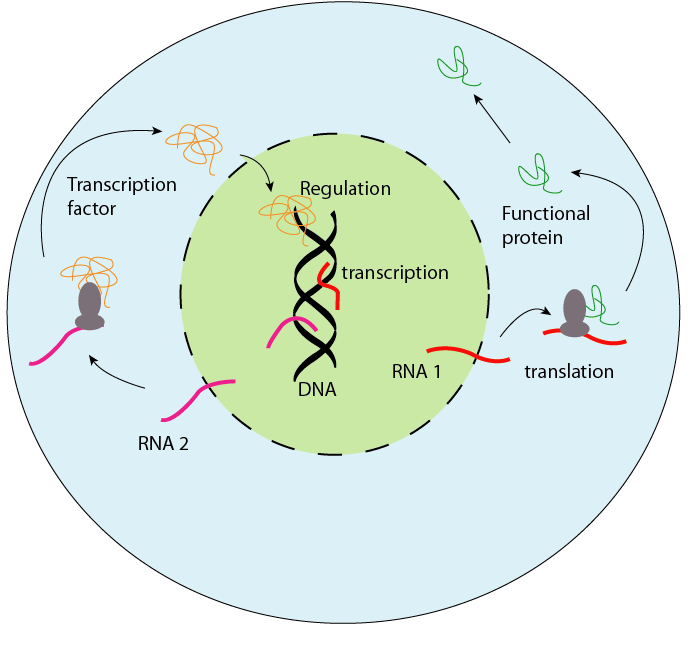
\includegraphics[width=.45\linewidth]{gfx/chapter1/cell.png}} \quad
        \subfloat[Differentiated neuron, with typical axons development.]
        {\label{fig:diff_cell}%
         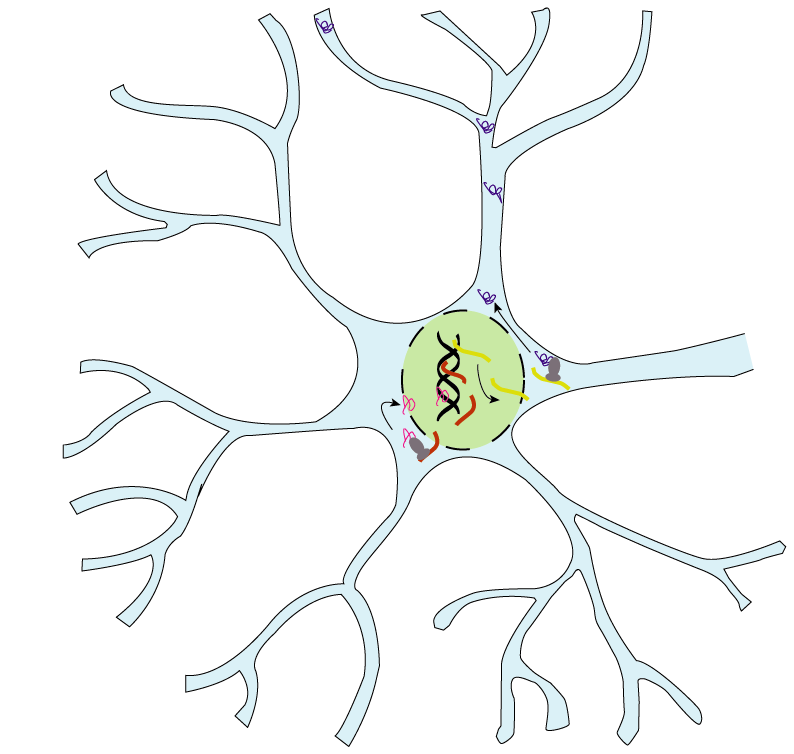
\includegraphics[width=.45\linewidth]{gfx/chapter1/neurone.png}}
        \caption{Cell types anatomical heterogeneity, gene expression and protein translation and gene regulatory networks. The schematics shows that genes in the DNA are transcribed to RNA molecules that are further translated outside the nucleus into proteins. Those proteins can serve various purposes inside the cell or come back to the nucleus to regulate gene expression.}\label{fig:cells}
\end{figure}
	
	During development, different mechanisms exist that allow gene expression to become differential as cell divisions occur. This is how the asymmetrical axis (dorso-ventral, and basal-apical) of the body are defined. One of the main mechanisms involves signalling gradients. The first of these gradients has to come from the zygote which must contain some asymmetrically distributed chemical so that the first divisions lead to non identical cells.\\
	
	Gene expression is one of the key factors during tissue development. Therefore, the ability to study gene expression patterns has revolutionized the field of developmental biology. Technological innovation has been the main driving factor of this revolution. In the next section I will present two methods for assaying gene expression.


\section{Capturing gene expression in the laboratory}\label{sec:gene_expression_lab}
     \subsection{In-situ hybridization assays}
     In-situ hybridization (ISH) is an experimental technique where the practitioner is able to determine in which cells of the tissue under study a particular RNA is present. As opposed to Southern blotting \cite{southern75}, ISH assays not only enable the experimentalist to know whether a gene is expressed or not, but also where in the tissue it is expressed. First proposed in 1969 by Pardue \cite{pardue69} and John \cite{john69} independently, in-situ hybridization (ISH) used radioactive tritium labelled probes on a photographic emulsion to reveal parts of the studied tissues where particular RNA or DNA sequences are present. With the development of fluorescent labelling techniques \cite{landegent84,pinkel88} allowing for faster, more sensitive and of course safer hybridization assays compared to radioactive probes \cite{swiger96}, Fluorescent in-situ hybridization (FiSH) quickly became the standard technique to study gene expression in the spatial context of biological tissues. Importantly, using multiple fluorescent probes of different colours allowed the simultaneous localization of several RNA fragments within a tissue \cite{nederlof89}.\\
     
     For small enough tissues to study, it is possible to stain hybridize the probes in the whole animal. This method called Wholemount in-Situ hybridization (WiSH) and a 3-Dimensional representation of the expression pattern of a gene can be deduced using confocal microscopy to study the patterns of gene expression slice by slice.
     

     \subsection{RNA sequencing}
     Whole Transcriptome Shotgun Sequencing (WTSS) also called RNA sequencing (RNA-seq) \cite{morin08,wang09} has developed alongside Next Generation Sequencing (NGS) techniques used to sequence genomic DNA. In RNA-sequencing, only the fraction of RNA molecules in the cell are targeted. Protein coding mRNA molecules can further be selected, they are separated from the rest by targeting the polyadenylated 3' tail, a characteristics exhibited by to protein coding transcripts and a few other types of transcripts only (lnc RNAs). Most current technique use magnetic beads to achieve this separation \cite{mortazavi08,morin08}.\\
     
    Once isolated from a population of cells, transcripts undergo fragmentation to obtain an average length of 200-300 nucleotides. The next step is the reverse transcription, which creates a complementary DNA (cDNA) library using viral reverse transcriptase enzymes. After amplification using quantitative Polymerase Chain Reaction (qPCR), the cDNA library is ready to be sequenced by NGS technology.\\
    
    The sequencing generates a large dataset of small reads, which need to be mapped back onto the reference genome of the considered species, providing this genome is available. In this case, the resulting dataset will reflect a snapshot of the whole transciptome in the studied cell population. In a case where the reference genome is not fully available, an alternative option is to map the reads back to a list of known gene sequences. The resulting dataset will represent a quantitative image of the considered genes in the cell population at one point in time.\\
    
    Because of technical limitations in this sequencing protocol, until very recently the starting quantity of RNA had to be relatively important (this issue is discussed further in \ref{sec:single_cell_rnaseq}). This is why most of the published RNA sequencing studies use a population of cell as a starting point. This however, means that the gene expression landscape obtained as an output will represent an averaged expression over all the cells used as an input.\\
    
    Importantly, when comparing RNA-seq to the previously described in-situ hybridization technique, if the methodological burden to analyse the expression of a lot of genes at the same time is greatly reduced, the spatial localisation of the cells is lost during the protocol.\\
    
    
\section{Platynereis dumerilii, an ideal organism for studying brain evolution}\label{sec:platynereis}
     \subsection{General description}
     \platyfull{} is a marine annelid of the class Polychaeta, which has been established as one of the main marine animal models in the fields of evolutionary, and developmental biology as well as ecology, toxicology and neurobiology \cite{hutchinson95,tessmar03,hardege99,dorresteijn90,fischer04,Fischer10}.\\
     
     \platy{} populates shallow (no more than 3m deep) ocean floors around the world. It is commonly found in the Mediterranean sea, the north Atlantic coast of Europe as well as in the shallow seas surrounding Sri Lanka, Java and the Philippines. Eggs, embryos and larvae are roughly 160$\mu$m long while the adults can measure up to 6cm in length.
     
     
\begin{figure}[bth]
        \myfloatalign
        \subfloat[Larval form of \platy{}. Image: MPI for Developmental Biology.]
        {\label{fig:platynereis_larvae}
        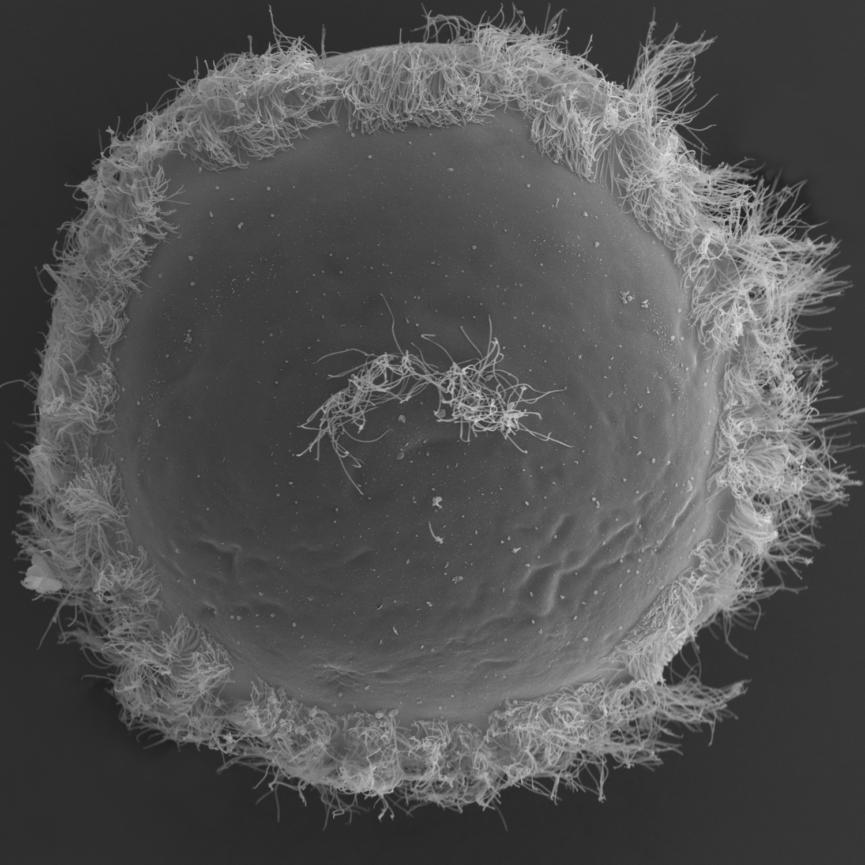
\includegraphics[width=.45\linewidth]{gfx/chapter1/platynereis_larva.jpg}} \quad
        \subfloat[Adult \platy{}. Image: Arendt group, EMBL]
        {\label{fig:platynereis_adult}%
         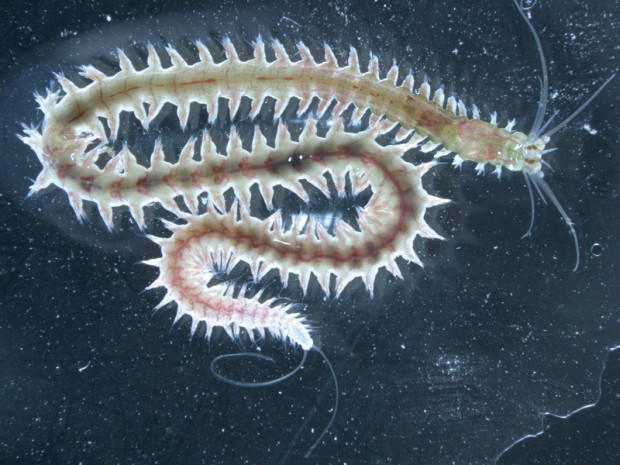
\includegraphics[width=.45\linewidth]{gfx/chapter1/platynereis_adult.jpg}}
        \caption{\platyfull{}'s larva and adult forms.}\label{fig:platynereis}
\end{figure}
     
     They are several reasons why \platy{} has been chosen as a model by numerous laboratories. Indeed, evolutionary wise, \platy{} shows several interesting characteristics.  As a member of the bilaterians \platy{} has a defined bilateral symmetry. It belongs to the lophotrochozoan taxon of the bilaterians as opposed to most of the well established model animals which either belong to the ecdysozoans (\species{Caenorhabditis elegans}, \species{Drosophila melanogaster}) or the deuterostomes (mouse, human). \platy{} as one of the only lophotrochozoan model is essential to be able to use comparative approaches full range of bilaterians \cite{Fischer10}.\\
     
     \platy{} also exhibits an exceptionally slow evolving nature. It has even been described as a ``living fossil" for that reason \cite{Fischer10}. Therefore, the numerous ancestral developmental characteristics exhibited by \platy{} translate into an image of the common past of all bilaterians. For example, an interesting example described in \cite{denes07,tessmar07} is the conserved molecular topography of the genes responsible for the development of the central nervous system between \platy{} and all vertebrates. This slow evolving nature makes \platy{} a better comparison with vertebrates than fast evolving species like \emph{Drosophila} and nematodes where derived features can obscure evolutionary signal \cite{Fischer10,arendt124}.\\
     
     Experimentally speaking, model organisms are chosen for several characteristics that make them easy to use in the laboratory, those characteristics include but are not limited to the size of the animal, the conditions required for the organism to develop, gestation and development time, ease to generate a new generation.\\
     
     in that regard \platy{} is nearly an ideal animal. Even in their adult form, they a relatively small, they can easily be kept and bred in captivity producing offspring throughout the year \cite{fischer04}. Furthermore, the behavioural characteristics of \platy{}'s mating ritual have been well studied and can be reproduced on demand in the laboratory. The ``nuptial dance" happens on the water surface. Males and females respectively release the sperm and eggs synchronously. This activity is synchronized by pheromones released into the water \cite{zeeck98}. Over 2000 individuals can be produced within a single batch. Every new individual will undergo embryonic then larval development before reaching \platy{}'s adult form.\\

 
     \subsection{Larval development}
    Similarly to the other polychaetes, the larval development of \platy{} can be decomposed into three main anatomical stages, as detailed in \cite{hauenschild69}: the trochophore, the metotrochophore and the nectochaete. The trochophore is spherical and moves thanks to an equatorial belt of ciliated cells as well as an apical organ displaying a ciliary tuft \cite{rouse99,nielsen04} as seen in Figure \ref{fig:platynereis_larvae} and schematically in Figure \ref{fig:platynereis_larvae_scheme}. The metotrochophore stage is characterized by the development of a slightly elongated segmented trunk compared to that of the trochophore \cite{hacker98}. The next developmental stage is referred to as the nectochaete larvae which resembles the adult (figure \ref{fig:platynereis_adult}) in many traits, especially with parapodial appendages used for swimming and crawling \cite{hacker98}.\\
    
\begin{figure}[bth]
\begin{center}
  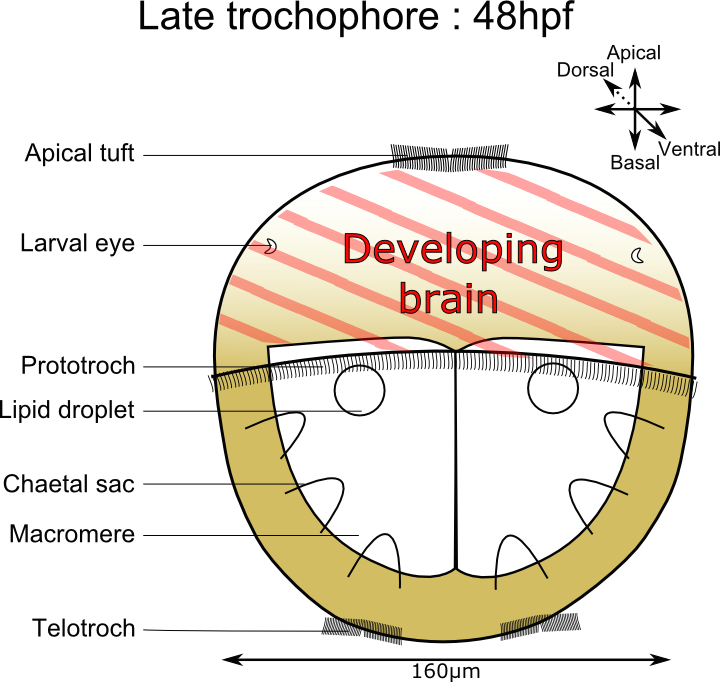
\includegraphics[width=0.6\linewidth]{gfx/chapter1/larvae48hpf.png}
\end{center}
  \caption{\platyfull{}'s larvea development at 48hpf (late trochophore). Red stripes indicate the area that forms the developing brain of the larvae.}
  \label{fig:platynereis_larvae_scheme}
\end{figure}
    
    Aside from this purely anatomical description, an additional staging system exists and has become the norm for current studies. The development is measured in \textit{hours post fertilization} (hpf) at $18^{\circ}C$.
    
    A key factor making \platy{} such an interesting model to work with is the fact that after fertilization, the $\approx 2000$ larva will start developing at the exact same time, in a synchronous fashion. Furthermore, the larval development of \platy{} follows a very stereotypical pattern with little variation from one individual to the other; this is true even between batches provided the temperature is kept constant \cite{fischer04,dorresteijn90}. An illustration of this synchronous development is shown in figure \ref{fig:brain_comparison}. This is a very important feature as it allows biologists to repeat experiments on several individuals at a very close developmental stage even if they are from different batches.\\
    
\begin{figure}[bth]
  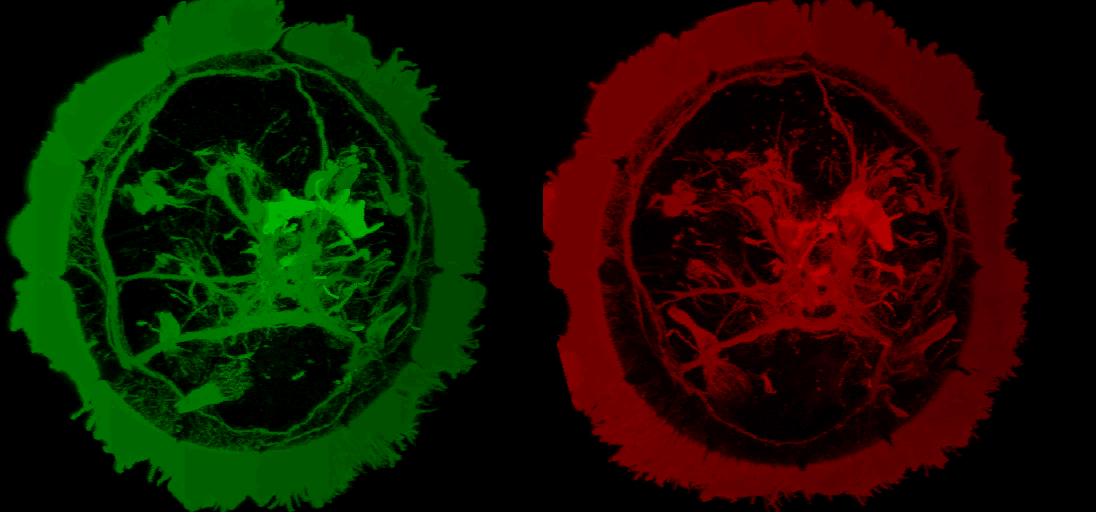
\includegraphics[width=\linewidth]{gfx/chapter1/brain_comparison.png}
  \caption{\platyfull{}'s stereotypical and synchronous development. In green and red are two different \platy{} individuals' with the same gene expression being highlighted (specifically, the target gene is \todo{find gene} highlighting the axonal scaffold). They show extremely similar patterns of development for the nervous system.}
  \label{fig:brain_comparison}
\end{figure}

	 
	  \subsection{Platynereis' nervous development until 48hpf}
	 Describing the entire development of \platy{} does not fall within the scope of this thesis. Indeed, I will only be interested in the brain of \platy{}'s larvae at 48hpf. Therefore, it is important to have an anatomical idea of what the brain looks like at this time in development and what inherent characteristics will be the most interesting to investigate. \platy{}'s larval brain development is detailed in \cite{Fischer10}.\\
     From the early trochophore (24-26hpf) neural system development starts taking place. The apical ganglion which contains one sertonergic cell and a few neurons linked to the nerve of the ciliary band of the larva called the prototroch forms at the apical tuft, (see Figure \ref{fig:platynereis_larvae_scheme}). This allows the first movements of the larvae thanks to the cialited cells of the prototroch.\\
     The mid-trochophore (26-40 hpf) sees the formation of the first cerebral commissure: a band of nerves interconnecting the ventral nerve cord and the brain, which is a typical feature of annelid neurobiology. During this phase the apical ganglion becomes bigger with three more serotonergic cells.\\
     The late trochophore (40-48hpf) sees the formation of the second commissure in the ventral nerve cord. It is at the end of this stage that the tissues of the brain become more complex with a notable increase in the number of neurites \cite{Fischer10}.\\
     The data used in the rest of this thesis will not encapsulate the whole larvae, just the developing brain (see figure \ref{fig:platynereis_larvae_scheme}) thus excluding the ventral part of the nervous system. The best studied areas of the developing brain are the larval eyes, the developing adult eyes and the apical organ on the dorsal side. On the ventral side are located the mushroom bodies, a pair of structures that are known to play a role in olfactory learning and memory in insects and annelids \cite{Tomer10}.\\
     
     Consequently, even at this early stage in a relatively ``simple" organism, the brain quickly becomes an extremely complex tissue. Cell types diverge and functional areas are formed. Before trying to understand more about \platy{}'s brain organization, it is interesting to ask the more general question of how complex tissues such as the brain are defined spatially.
     
     \subsection{Building a image library of gene expression for Platynereis}
     During his PhD, Raju Tomer and other \todo{cite thesis} members of the Arendt lab in EMBL, used wholemount in-situ hybridization to create an image library of gene expression in the brain of \platy{}. They were able to record gene expression in the full brain at 48hpf for 169 genes. In practice, each individual larvae was dissected to isolate the region containing the developing brain. Each brain was then stained with two different fluorescent probes corresponding to two messenger RNAs (mRNA). One of the genes is considered a reference, as it is always hybridized in all the assays (the main reference gene used was Emx) alongside another gene of interest, see figure \ref{fig:insitu}. Each brain was then visualized with laser confocal microscopy to reveal the gene expression patterns in the brain slice by slice, generating at the same time 3D coordinates for each slice.\\
     
     As mentioned previously, the larval development of \platy{} is highly similar in every individual larvae. In the case of this study where WiSH was performed on many independent animals, the stereotypical development of \platy{} has proven essential. Indeed, having the same reference gene localized in all assays allowed Tomer to align all other gene expression patterns onto this scaffold. The result is an image library of 169 gene expression patters in the full brain of \platy{} with a exploitable spatial reference that allows for a very precise mapping.\\
    
    \begin{figure}[bth]
\centerline{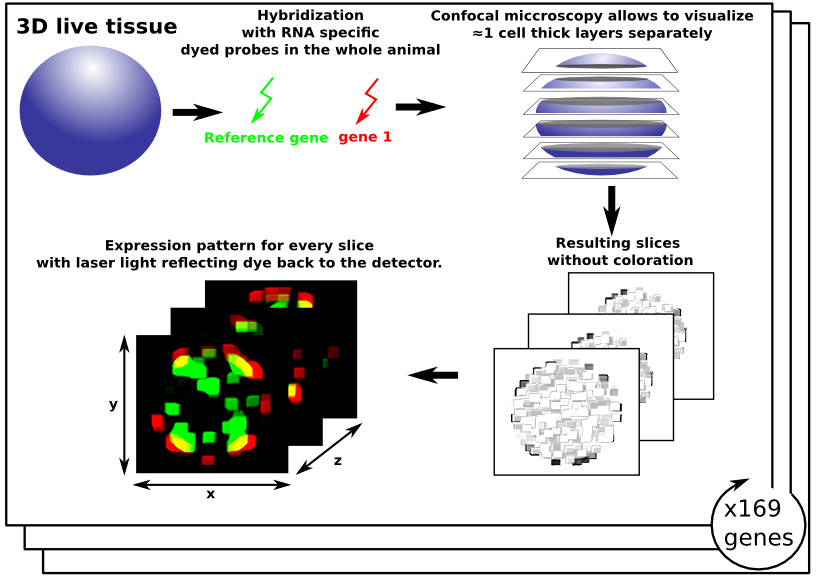
\includegraphics[width=0.9\linewidth]{gfx/chapter1/insitu.png}}
\caption{Wholemount in-situ hybridization ssays used to create a 169 genes catalogue of gene expression in the brain of \platy{}. From the live tissue cut into thin fixed layers, every slice is stained with a reference gene and a gene of interest that will reveal areas of expression under fluorescent microscopy. The process repeated 169 times for key genes in \platy{} neural development has been generated by \cite{Tomer10}}\label{fig:insitu}
	\end{figure}
	
	However useful and practical WiSH may be, such assays are limited in terms of the number of genes one is able to study. Indeed, each individual larvae only provides the expression of two genes, one being the reference. To overcome this problem, crucial developments in sequencing technologies have brought about a new way of studying the expression of the whole transciptomic landscape in a single assay,namely RNA sequencing.


    
\section{Summary}
     
     

	In the introduction, I have presented one extremely important aspect of cell and developmental biology, namely, gene expression. I have given an overview of how cells express their genomes and what how the expression of specific signalling genes can influence the fate of cells during development. I have also described two methods that allow practitioners to capture gene expression from a biological tissue: in-situ hybridization and RNA-seq.\\
	
	Subsequently, I described \platyfull{} and the advantageous traits it exhibits for developmental biologists especially in the field of neural development. I have discussed the fact that anatomical traits are not sufficient to fully comprehend the deep heterogeneous patterns of functionalities inside a complex organ such as the brain. In order push this understanding further I have discussed how gene expression levels can be used to characterise different tissues and how an image library of gene expression for 169 gene was generated by \cite{Tomer10} in the full brain of \platy{} using WiSH.\\
	
	So far, I have considered biology at the scale of the tissue, or the sub-tissue. However, the heterogeneity of complex biological tissues does not stop at this scale of study. In fact, with a top-down approach looking at big tissues and then separating them in smaller sub-tissues until ``true" functional tissues are defined is an extremely complicated problem. A solution to this problem would be to reverse the approach from a top-down to a bottom-up mindset. This means reducing the scale of study to the smallest biological unit available, the single cell, defining the heterogeneity of gene expression at the single cell level and going back up to the functional tissue level from there. Instead of a fragmentation problem, this becomes a clustering problem, attaching single cells to a certain number of categories. In order to implement such an approach, single cell gene expression data is therefore needed.\\
	
	This model animal, the image library of gene expression in its brain and the question of finding functional tissues and sub-tissues from single cell gene expression are the key concepts that motivate this thesis.\\
	
	In the first chapter I will describe how advances in both RNA-seq and in-situ hybridization have allowed the extraction of single cell gene expression data and how this data is analysed. I will also describe how an ``ideal" dataset of spatially referenced single cell expression data can potentially be create by mapping the results of single cell RNA-seq onto an in-situ hybridization scaffold.\\
	
	in the second chapter I will present a tool I developed to allow an easy visualization of 3D information and more specifically clustering results. This tool will be central to the upstream and downstream analysis of the data and the results used in the thesis.\\
	
	

%
%
%
%
%



